\subsection{Data Modeling and Article Extraction}
The first phase in the program consists in parsing the article streams and producing the data structures needed in the subsequent steps. Though conceptually simple, the parsing has been challenged by several practical constraints. We will first give an overview of the data generated in this phase, and then a more technical description of the processing steps. Lastly, we will describe the practical problems we encountered and how we dealt with them.

\subsubsection{Data description}
The dataset is a collection of 159 years worth of articles for the \emph{Gazette de Lausanne} and 156 for the \emph{Journal de Genève}. The period starts from 1840 and ends in 1998 for both newspapers. The format of the data is a one-liner XML file per year and per newspaper. The root node contains one \textit{article} node per article, themselves containing one or several \textit{entity}'s per article part (if the article spans over multiple pages, for exemple). Each entity contains the associated article in plain text and all the metadata related to the article. The ones we used for our application were the \textit{issue date}, \textit{page number}, \textit{title} and \textit{publication}. The plain text is the result of an OCR scan of the original newspaper archive. Consequently, it is very noisy and contains lots of character recognition mistakes.
The total size of the dataset is 7.1 Go and 9.6 Go for the \emph{Gazette de Lausanne} and \emph{Journal de Genève} collections respectively.

\subsubsection{Parser output overview}
During such a long period, the French language has been subject to a progressive drift. In a way, the streams are composed of slightly different idioms which belong to particular temporal slices. Typically, a word like "Internet" only appears in the later part of the streams. In our project, this could potentially create a bias because of the background model, a structure described below. In order to compensate this, the program will not analyze the entire dataset, but a temporal subset which we define as the \emph{time frame}. Consequently, from the program's "perspective", the time frame acts as the dataset, so we will use this term instead when there is no ambiguity.
The \emph{background model} is an unique object on the whole dataset (i.e time frame). It allows to retrieve the distribution of every distinct word in the dataset. This structure is used during the theme analysis to determine how common a word is. At the time we needed to fine-tune our algorithms, it came out that having a \emph{background model} on a larger temporal subset than the time frame could improve results. Therefore, we defined a new time period type called  \emph{background model time frame}.
For the next part, we will differentiate two different phases in the processing pipeline: the theme extraction, where we perform the Expectation-Maximization (EM) algorithm, and the theme "strength" analysis, which uses the Hidden Markov Models (HMM). Both phases are described later. For the EM phase, the parser has to provide a structure containing the word count inside each individual article text. For that, we use an object representing a \emph{parsed article}, which contains the count of each distinct word in this article, as well as some other properties (issue date, stream identifier...). These parsed articles must be grouped by small sub-partitions of the time frame that we called \emph{time partition}s. Effectively, the EM part receives an RDD of \emph{time partition}s containing a small part of the parsed articles. The HMM part requires the chronological concatenation of all the words in the \emph{time frame} , where a timestamp is attributed to each word. In order to reduce the memory and CPU usage of such a structure, we don't store the words as Java String objects; rather, we first associate each distinct word to a unique integer identifier, and then produce the word concatenation as an ordered RDD of integers. Both the EM and HMM parts need to access the background model. Figure \ref{fig:time_entities} summarizes the different time entities we defined.

\begin{figure}
   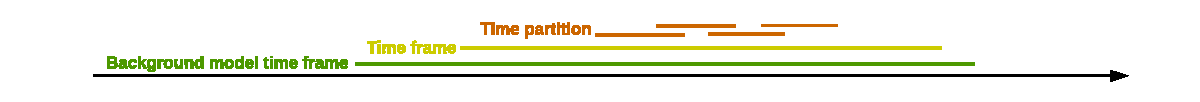
\includegraphics[width=\textwidth]{time_entities.pdf}
   \caption{\label{fig:time_entities} The different types of time periods on a time-line.}
\end{figure}

\subsubsection{Data processing pipeline}
The parser does not produce all its output on a single method call. The background model must be computed at the beginning, but the input provided for the EM and HMM parts are generated "on demand", in order to avoid storing pending data (we don't want to keep the HMM input for the whole execution, only to use it once at the end). However, it would be expensive to parse and transform the XML files from scratch at each of these steps. Instead, we produce an intermediary RDD from which all these outputs can be derived. First, we parse the XML streams, retrieve the articles, and segment their text content into a list of words. This list, along with other informations about the article like the issue date and the title, are stored in a container we named \emph{segmented article}, which is accumulated in our base RDD.
The background model is generated immediately after this base RDD is computed.
We generate the EM phase input on demand by associating each word to its number of occurrences inside every segmented article individually. Using a provided partitioning of the \emph{time frame} into \emph{time partitions}, the parser returns the RDD of grouped parsed articles.
Finally, for the HMM phase, we first use the background model to build a lexicon that translates each unique word into an integer identifier. The segmented articles are then sorted chronologically, after what we extract their lists of words, translate them into lists of identifiers using the lexicon, and assemble all the results in one single RDD. This is done on demande by a method call at the time we run the HMM phase.
It is noticeable that some of these operations are quite redundant. Part of this problem is due to the fact that we are exposed to a "chicken-and-egg" situation; the background model must be produced from the list of extracted articles, but we also need the background model during the processing of the article RDDs (and not only for the HMM phase as we will see in the next section). Because of this, and other optimizations that we describe below, we inevitably apply similar transformations over the whole dataset. Nevertheless, all of the operations are particularly simple and can be fully parallelized, resulting in a satisfying total execution time.

\begin{figure}
   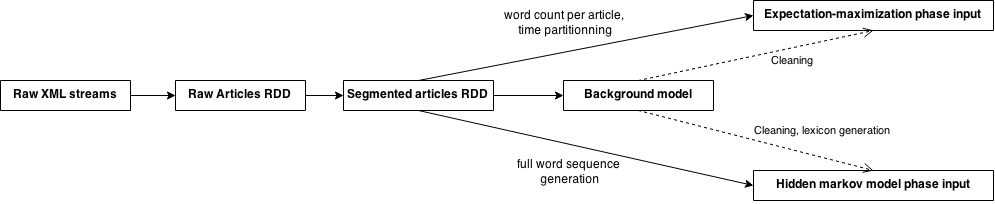
\includegraphics[width=\textwidth]{parser_processing_steps.png}
   \caption{\label{fig:parser_processing_steps} Parser processing pipeline}
\end{figure}

\subsubsection{Data cleaning and filtering}
The parser also enable some basic cleaning and filtering functionality. There was two main factor for noise introduction: OCR errors and meaningless (for us) articles. The problem with OCR errors is that they make the size of the \emph{background model} grow linearly with the \emph{background model time frame} length because of the "new" words they introduce. This is a problem because the \emph{background model} needs to fit in main memory and is queried very frequently. The adopted solution is to set a threshold on the word frequency. Word above the given frequency are simply discarded from the articles and the \emph{background model}. This way, unusual OCR error are discarded, while the usual ones are part of the \emph{background model} so that they do not disturb later stages.
To address the meaningless articles problem, we can set two parameters at parse time. The first is a threshold on the number of word per article. Articles having count above this threshold are discarded. The second is the page number threshold. It filters out article that begins at page greater than the threshold. The problem with this is: it is not always the case that article on the first pages are the most relevant ones as we are used to.
In fact, setting those parameters is very tricky and depends on the \emph{time frame} of interest. Better understanding of written press at this time is in fact needed to accomplish this.
